%% ══════════════════════════════════════════════════════════════
%%  CHAPTER 2 — SYSTEM ARCHITECTURE
%% ══════════════════════════════════════════════════════════════
\chapter{System Architecture}
\label{ch:architecture}

\section{High-Level Architecture}
\label{sec:arch:high-level}

\autoscholar follows a three-tier architecture with a React \gls{spa} frontend, a Node.js/Express backend, and a SQLite/PostgreSQL persistence layer.
The AI reasoning engine (\claude) operates as an external service accessed via the Anthropic HTTP API, while Python computational services run as short-lived subprocesses.

The defining architectural characteristic is the \textbf{streaming tool-execution loop}: the backend maintains a long-lived \gls{sse} connection with the client while simultaneously conducting a multi-turn conversation with Claude.
Each turn may involve Claude issuing one or more tool calls, the server executing them (potentially spawning Python subprocesses, calling external APIs, or querying databases), and returning the results to Claude for the next reasoning step.
This loop can execute up to 180 tool calls in a single auto-paper run.

\begin{figure}[H]
\centering
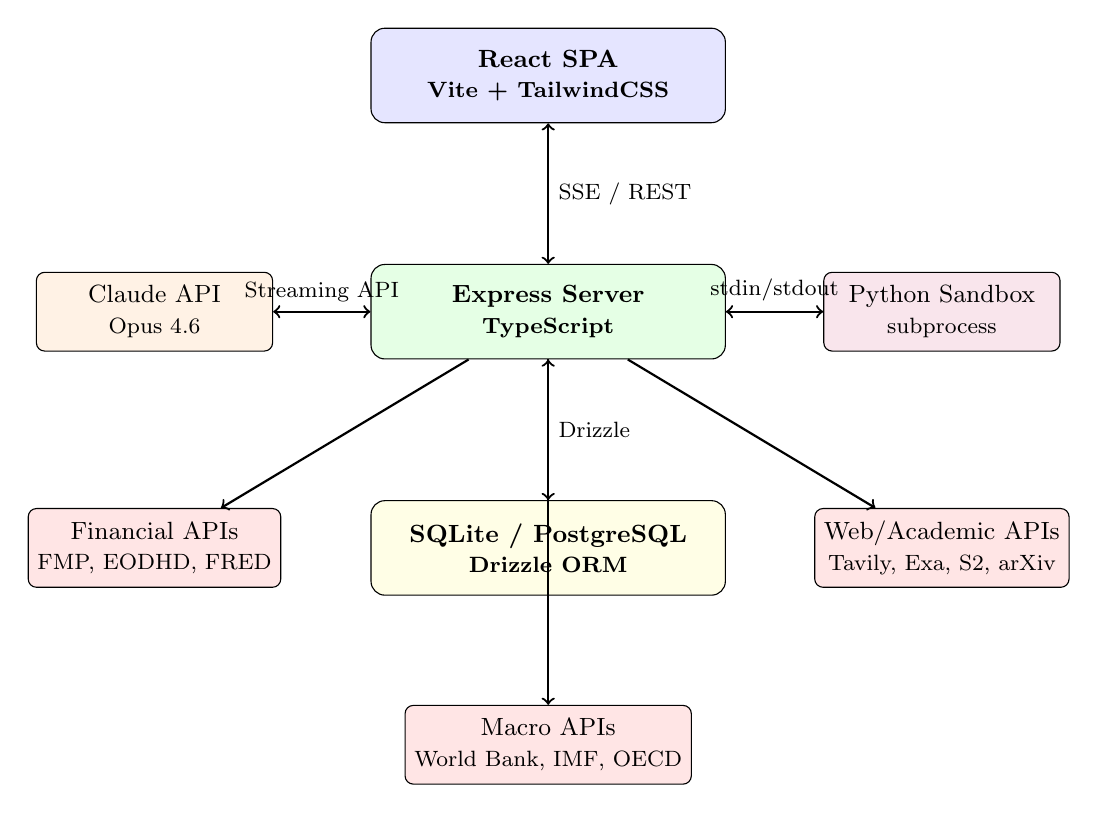
\begin{tikzpicture}[
  box/.style={draw, rounded corners=3pt, minimum width=3cm, minimum height=1cm, align=center, font=\small},
  bigbox/.style={draw, rounded corners=5pt, minimum width=4.5cm, minimum height=1.2cm, align=center, font=\small\bfseries},
  arrow/.style={->, thick},
  darrow/.style={<->, thick},
]

% Client tier
\node[bigbox, fill=blue!10] (client) at (0,6) {React SPA\\{\footnotesize Vite + TailwindCSS}};

% Server tier
\node[bigbox, fill=green!10] (server) at (0,3) {Express Server\\{\footnotesize TypeScript}};

% External services
\node[box, fill=orange!10] (claude) at (-5,3) {Claude API\\{\footnotesize Opus 4.6}};
\node[box, fill=purple!10] (python) at (5,3) {Python Sandbox\\{\footnotesize subprocess}};

% Data tier
\node[bigbox, fill=yellow!10] (db) at (0,0) {SQLite / PostgreSQL\\{\footnotesize Drizzle ORM}};

% External APIs
\node[box, fill=red!10] (finapi) at (-5,0) {Financial APIs\\{\footnotesize FMP, EODHD, FRED}};
\node[box, fill=red!10] (webapi) at (5,0) {Web/Academic APIs\\{\footnotesize Tavily, Exa, S2, arXiv}};
\node[box, fill=red!10] (macroapi) at (0,-2.5) {Macro APIs\\{\footnotesize World Bank, IMF, OECD}};

% Arrows
\draw[darrow] (client) -- node[right, font=\footnotesize] {SSE / REST} (server);
\draw[darrow] (server) -- node[above, font=\footnotesize] {Streaming API} (claude);
\draw[darrow] (server) -- node[above, font=\footnotesize] {stdin/stdout} (python);
\draw[darrow] (server) -- node[right, font=\footnotesize] {Drizzle} (db);
\draw[arrow] (server) -- (finapi);
\draw[arrow] (server) -- (webapi);
\draw[arrow] (server) -- (macroapi);

\end{tikzpicture}
\caption{High-level system architecture of \autoscholar.}
\label{fig:high-level-arch}
\end{figure}

\section{Component Map}
\label{sec:arch:components}

The server-side codebase is organized into five major component groups, each with distinct responsibilities:

\subsection{Entry Points and Configuration}

\begin{description}
  \item[\file{server/index.ts}] (187 lines) --- The application entry point. Initializes Express with CORS, session management (SQLite or PostgreSQL session store), request logging, route registration, and Vite dev server or static file serving. On startup, it initializes the \gls{asid} system and launches the auto-paper scheduler. Installs global handlers for \texttt{unhandledRejection} and \texttt{uncaughtException} to prevent server crashes.

  \item[\file{server/routes.ts}] (34 lines) --- Central route registration hub. Imports and mounts 8 route modules (chat, auth, admin, analytics, FMP, reports, prompts, public API) and schedules periodic cleanup of stale \LaTeX{} compilations every 30 minutes.

  \item[\file{server/db.ts}] (241 lines) --- Database abstraction layer supporting three backends: SQLite via \pkg{better-sqlite3}, local PostgreSQL via \pkg{pg}, and Neon Serverless PostgreSQL. For SQLite, performs extensive inline schema migrations (creating 10+ tables, adding columns via safe \texttt{ALTER TABLE} statements). Exports a unified Drizzle \gls{orm} instance and raw database pool.

  \item[\file{server/storage.ts}] (1 line) --- Barrel re-export pointing to the composed storage singleton.
\end{description}

\subsection{Route Handlers}

The routing layer is organized into three tiers:

\begin{enumerate}
  \item \textbf{Core routes} --- \file{routes/chat.ts} (1,066 lines), \file{routes/admin.ts} (675 lines), \file{routes/auth.ts} (189 lines), \file{routes/fmp.ts} (317 lines), \file{routes/prompts.ts} (41 lines).

  \item \textbf{Report sub-routes} --- 9 modules in \file{routes/reports/} covering document generation, journal papers, DOI/ASID management, figures, peer reviews, shared reports, sessions, platform stats, and the repository browser.

  \item \textbf{Public API v1} --- 9 modules in \file{routes/api/v1/} providing authenticated access to papers, reviews, reports, stats, pipeline monitoring, search, prompts, sessions, and key management.
\end{enumerate}

The single largest route file is \file{routes/toolExecutor.ts} at 2,945 lines, containing the massive dispatch function that maps Claude's tool call names to their service implementations.

\subsection{Service Layer}

Services are organized by domain:

\begin{longtable}{lp{8cm}r}
\caption{Service modules by domain.} \label{tab:services} \\
\toprule
\textbf{Domain} & \textbf{Key Modules} & \textbf{Lines} \\
\midrule
\endfirsthead
\toprule
\textbf{Domain} & \textbf{Key Modules} & \textbf{Lines} \\
\midrule
\endhead
Claude/AI & \file{claude/systemPrompt.ts}, \file{claude/claudeStreaming.ts}, \file{claude/tokenManagement.ts}, \file{claude/tools/} (13 files) & $\sim$9,900 \\
Python Computation & \file{python/customPythonExecutor.py}, \file{python/customPython.ts}, plus 9 service pairs (GARCH, VaR, Monte Carlo, portfolio, risk, volatility surface, options, data download, plots) & $\sim$8,500 \\
\LaTeX{} Engine & \file{latex/paperGenerator.ts}, \file{latex/compiler.ts}, \file{latex/sanitizer.ts}, \file{latex/latexPatchManager.ts}, \file{latex/latexLogParser.ts}, \file{latex/packaging.ts} & $\sim$2,870 \\
Governor & \file{governor/governorEngine.ts}, \file{governor/types.ts}, \file{governor/promptProfiles.ts}, \file{governor/jfWritingStyle.ts}, \file{governor/academicFigureStyle.ts} & $\sim$1,507 \\
Financial Data & \file{fmp/} (15 files), \file{eodhd\_service.ts}, \file{financialDataService.ts} & $\sim$2,000 \\
Web/Academic & \file{academicSearchService.ts}, \file{tavilyService.ts}, \file{exaService.ts}, \file{firecrawlService.ts}, \file{serpapiService.ts} & $\sim$2,160 \\
Macro & \file{worldBankService.ts}, \file{imfService.ts}, \file{oecdService.ts} & $\sim$320 \\
Pipeline & \file{autoPaperScheduler.ts}, \file{researchPaperService.ts}, \file{peerReviewService.ts}, \file{literatureGapFinderService.ts} & $\sim$2,310 \\
Other & \file{webDatasetService.ts}, \file{doiService.ts}, \file{polymarketService.ts}, \file{promptBank.ts}, \file{figureAnalysisService.ts}, \file{sessionBroadcaster.ts}, \file{cryptoDonationService.ts} & $\sim$2,300 \\
\bottomrule
\end{longtable}

\subsection{Storage Layer}

The storage layer is decomposed into 6 domain-specific modules:

\begin{itemize}
  \item \file{storage/user-storage.ts} --- User CRUD with cascading session deletion.
  \item \file{storage/message-storage.ts} --- Chat messages and shared reports.
  \item \file{storage/session-storage.ts} --- Conversation session lifecycle.
  \item \file{storage/paper-storage.ts} --- Published papers, pipeline runs, and cost tracking.
  \item \file{storage/analytics-storage.ts} --- Active users, metrics, and request logs.
  \item \file{storage/admin-storage.ts} --- Governor state, peer reviews, donations, API keys, site config.
\end{itemize}

These are composed into a single \texttt{storage} object via the barrel file \file{storage/index.ts}, implementing the 70+ method \texttt{IStorage} interface.

\subsection{Shared Types and Schema}

The \file{shared/} directory contains:

\begin{itemize}
  \item \file{schema.ts} (357 lines) --- PostgreSQL Drizzle schema defining 20 tables.
  \item \file{schema-sqlite.ts} (456 lines) --- SQLite Drizzle schema (canonical superset, includes \texttt{apiKeys} table).
  \item \file{types.ts} (44 lines) --- Shared API contract types used by both client and server.
\end{itemize}

\section{Data Flow Architecture}
\label{sec:arch:dataflow}

\subsection{Interactive Chat Flow}

The interactive chat flow follows this sequence:

\begin{enumerate}
  \item The client sends a POST to \texttt{/api/chat} with the query, conversation history, optional image/data, and session ID.
  \item The server validates the request via Zod schemas (\file{routes/validation.ts}).
  \item If the query matches a research paper pattern, it is upgraded via \func{upgradeResearchPrompt} using Claude Opus.
  \item The system prompt is built via \func{buildSystemPrompt} (1,798 lines), incorporating the current date, author profile, and research context.
  \item \func{callClaudeStreamingWithRetry} initiates the streaming conversation with up to 5 retries on transient failures.
  \item For each response chunk:
    \begin{itemize}
      \item Text deltas are forwarded to the client via SSE.
      \item Tool calls trigger \func{executeToolCall} (2,945-line dispatch), which routes to the appropriate service.
      \item Tool results are sent back to Claude for the next turn.
    \end{itemize}
  \item Session data (messages, tool results, figures) is persisted every 8 seconds.
  \item On completion, final session state is saved and the SSE stream is closed.
\end{enumerate}

\subsection{Auto-Paper Pipeline Flow}

The autonomous pipeline adds several layers on top of the interactive flow:

\begin{enumerate}
  \item The scheduler (\file{autoPaperScheduler.ts}) selects a prompt from the 1,000+ entry prompt bank.
  \item A pipeline run is created in the database with status \texttt{queued}.
  \item The pipeline internally calls the same \texttt{/api/chat} endpoint as a client.
  \item A \governor engine monitors tool results and injects directives.
  \item On completion, \popper validates the paper via AI peer review.
  \item Papers scoring $\geq 45/100$ are published; below that threshold they are rejected.
  \item The run status is updated to \texttt{published}, \texttt{rejected}, or \texttt{failed}.
\end{enumerate}

\section{Execution Model}
\label{sec:arch:execution}

\subsection{Streaming SSE Protocol}

All chat communication uses Server-Sent Events with the following event types:

\begin{table}[H]
\centering
\caption{SSE event types in the streaming protocol.}
\label{tab:sse-events}
\begin{tabularx}{\textwidth}{lX}
\toprule
\textbf{Event Type} & \textbf{Description} \\
\midrule
\texttt{text} & Incremental text delta from Claude's response. \\
\texttt{sources} & Array of web search results with titles, URLs, and snippets. \\
\texttt{done} & Stream completion signal with final session ID and token usage. \\
\texttt{error} & Error message (transient or fatal). \\
\texttt{python\_code} & Python code executed, with script ID and description. \\
\texttt{python\_figures} & Base64-encoded matplotlib figures from Python execution. \\
\texttt{python\_output} & Captured stdout from Python scripts. \\
\texttt{tool\_result} & Structured result from a tool execution (name, summary, data). \\
\texttt{search\_query} & Search query dispatched to an external API. \\
\texttt{agent\_step} & Pipeline progress indicator (agent name, step, status). \\
\texttt{monte\_carlo} & Monte Carlo simulation results (paths, statistics). \\
\texttt{options\_pricing} & Black-Scholes pricing results with Greeks. \\
\texttt{download\_link} & URL for a generated file (CSV, XLSX, PDF, ZIP). \\
\texttt{section\_written} & Research paper section committed (title, word count). \\
\texttt{paper\_compiled} & Final paper PDF URL and compilation status. \\
\texttt{retry} & Retry attempt notification (attempt number, delay). \\
\bottomrule
\end{tabularx}
\end{table}

\subsection{Token Management}

The system operates within Claude's 1M-token context window using several strategies:

\begin{description}
  \item[Token estimation.] A 4-characters-per-token heuristic (\func{estimateTokens}) provides fast approximate counts without tokenizer overhead.
  \item[Tool result truncation.] Results exceeding 15,000 characters are truncated with a notice, applied selectively to prevent context overflow from large API responses.
  \item[History summarization.] When estimated message tokens exceed the 500K safety threshold, the system calls Claude to compress older conversation history into a summary, preserving key findings while freeing context space.
  \item[Cost tracking.] Real-time cost calculation using model-specific pricing (Opus 4.6: \$5/\$25 per MTok for input/output) enables budget monitoring.
\end{description}

\subsection{Concurrency Model}

The Express server runs in a single Node.js event loop.
Concurrency is achieved through:

\begin{itemize}
  \item \textbf{Async I/O:} All external API calls use \texttt{async/await} with \pkg{axios}, allowing multiple concurrent HTTP requests.
  \item \textbf{Python subprocesses:} Computational tasks spawn child processes via \texttt{child\_process.spawn}, running in parallel with the Node.js event loop.
  \item \textbf{Pipeline parallelism:} The auto-paper scheduler supports up to 3 concurrent paper generations via the \texttt{maxParallel} configuration parameter.
  \item \textbf{Parallel search:} Academic search functions run all 5 sources (Semantic Scholar, OpenAlex, arXiv, CrossRef, Google Scholar) concurrently via \texttt{Promise.allSettled}.
\end{itemize}

\section{Dependency Graph}
\label{sec:arch:dependencies}

The internal dependency structure follows a layered pattern:

\begin{figure}[H]
\centering
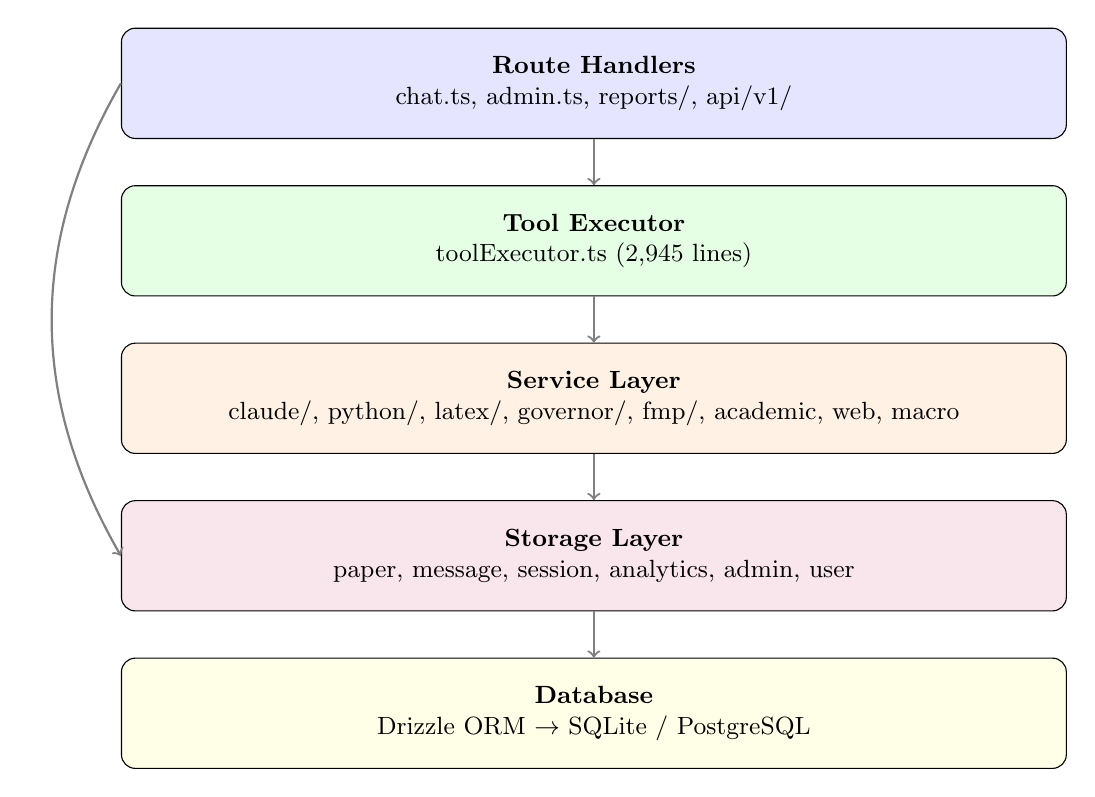
\begin{tikzpicture}[
  layer/.style={draw, rounded corners=5pt, minimum width=12cm, minimum height=1.4cm, align=center, font=\small},
  arrow/.style={->, thick, gray},
]

\node[layer, fill=blue!10] (routes) at (0,8) {\textbf{Route Handlers}\\chat.ts, admin.ts, reports/, api/v1/};
\node[layer, fill=green!10] (exec) at (0,6) {\textbf{Tool Executor}\\toolExecutor.ts (2,945 lines)};
\node[layer, fill=orange!10] (services) at (0,4) {\textbf{Service Layer}\\claude/, python/, latex/, governor/, fmp/, academic, web, macro};
\node[layer, fill=purple!10] (storage) at (0,2) {\textbf{Storage Layer}\\paper, message, session, analytics, admin, user};
\node[layer, fill=yellow!10] (db) at (0,0) {\textbf{Database}\\Drizzle ORM $\to$ SQLite / PostgreSQL};

\draw[arrow] (routes) -- (exec);
\draw[arrow] (exec) -- (services);
\draw[arrow] (services) -- (storage);
\draw[arrow] (storage) -- (db);
\draw[arrow, bend right=30] (routes.west) to (storage.west);

\end{tikzpicture}
\caption{Layered dependency structure.}
\label{fig:dependency-layers}
\end{figure}

\section{Security Architecture}
\label{sec:arch:security}

Security is implemented at multiple levels:

\begin{description}
  \item[Authentication.] Session-based authentication with SHA-256 + salt password hashing. Admin access requires a separate password. API keys use SHA-256 hashing with raw key visible only at creation.
  \item[API key obfuscation.] User-provided Anthropic API keys are stored using XOR obfuscation with the session secret, preventing plain-text storage in the database.
  \item[Rate limiting.] Per-key in-memory rate limiting for the public API (default 100 requests/hour) with automatic cleanup every 10 minutes.
  \item[Python sandboxing.] Python execution runs in subprocess isolation with JSON stdin/stdout protocol, no filesystem write access outside designated directories.
  \item[Input validation.] Zod schemas validate all request bodies. Tool inputs are schema-validated by Claude's tool-use protocol.
  \item[CORS.] Origin-restricted CORS allowing only \texttt{localhost} and \texttt{autoscholar.ai} domains.
\end{description}

\section{Configuration Management}
\label{sec:arch:config}

System configuration uses a three-tier approach:

\begin{enumerate}
  \item \textbf{Environment variables} (\file{.env}) --- API keys, database URLs, passwords, feature flags.
  \item \textbf{Database configuration} (\texttt{site\_config} table) --- Runtime-adjustable settings (scheduler cadence, Popper threshold, custom system prompt overrides).
  \item \textbf{Code constants} --- Model selection (\file{streamingConfig.ts}), token limits, retry parameters, prompt profiles (\file{governor/promptProfiles.ts}).
\end{enumerate}

\section{Deployment Model}
\label{sec:arch:deployment}

\autoscholar supports two deployment modes:

\begin{description}
  \item[Development.] Vite dev server with HMR for the frontend, \pkg{tsx} for TypeScript server execution, SQLite for zero-configuration database. All runs locally with \texttt{npm run dev}.
  \item[Production.] Vite builds the frontend to \texttt{dist/public/}, \pkg{esbuild} compiles the server to \texttt{dist/index.js}, and the app runs as a single Node.js process serving both the API and static files. Production typically uses Neon Serverless PostgreSQL.
\end{description}

The CI pipeline (\file{.github/workflows/ci.yml}) runs linting, type checking, and tests on push.
